\section{DEMONSTRATION}
\label{sec:demonstration}
% a simple tool for multiple choice dataset evaluation and correction
%\subsection{Setup}
%\KZ{Where is the demo on the web? URL?} 
We demonstrate our framework 
%with real-world and researchers can apply it to test 
%whether a test dataset is comprehensive or not 
%and evaluate a model from various aspects online.
%~\footnote{http://adapt.seiee.sjtu.edu.cn:3308/data\_traning/dataset}}, 
with 12 popular text inference datasets and 3 popular deep neural models.
The datasets can be 
classified into two types. 
The first type is NLI classification tasks (SNLI, QNLI, MNLI).
%a special case of multiple choice datasets. 
The second type is the multiple choice problems with one 
right sentence choice and uncertain wrong choices, 
%\KZ{Just call them MCQ? Is there a better name?} 
including ARCT, 
ARCT\_adv\cite{schuster2019towards}, 
RACE~\cite{lai2017race}, RECLOR~\cite{yu2020reclor}, 
%in which ``hypothesis'' 
%s one of the alternatives and ``premise'' contains more 
%than one context roles. 
Ubuntu~\cite{lowe2015ubuntu}, COPA~\cite{roemmele2011choice}, ROCStory, SWAG~\cite{zellers2018swag} and 
CQA~\cite{talmor2019commonsenseqa}.
%also belong to the second type but with only context role  in ``premise''. 
The models are fastText~\cite{joulin2017bag}, ESIM~\cite{chen2016enhanced} and BERT (base). 
In our system, we have trained 36 models (12 datasets and 3 models). Users can get the profiling 
results directly on this models. 
%We set $k = 10$, which means for Word feature, we only consider 
%top 10 words with highest feature scores \KZ{Where did we mention feature
%scores in Sec 3?}. 
Special care should be taken when using the Word feature. 
If the frequency of a word is too low, there will be very few cases 
for testing this feature. 
Thus we set the frequency threshold $\sigma$ to 5. 

%With ICQ, we managed to find some cues which affect the 
%three models. Some of them are shown in \secref{sec:model}. 
%User can try other features or even upload their own dataset or their own
%model (in the form of a prediction result file). 
%\KZ{How to try other features? did you mean define other features?}
%Special care should be taken when using the Word feature. 
%If the frequency of a word is too low, there will be very few cases 
%for testing this feature. We considered this 
%problem and experimented with different thresholds and 
%concluded that only words with frequency greater than 100 in the training data
%will qualify as a feature. This frequency is the sum number of a feature.

%\subsection{Scenarios}
%The demo will showcase the following scenarios.

%\subsubsection{Dataset Evaluation}

\begin{figure}[th]
\centering

\includegraphics[width=1.0\columnwidth]{picture/dataset1.eps}
\caption{Web UI of ICQ with existing datasets.}% \KZ{Make the fonts a bit bigger}}
\label{fig:dataset1}
\end{figure}

\begin{figure}[th]
\centering
\includegraphics[width=1.0\columnwidth]{picture/dataset.eps}
\caption{Web UI of ICQ with new datasets}% \KZ{Make the fonts a bit bigger}}
\label{fig:dataset}
\end{figure}

%\KZ{The following needs to be rewritten as the fig is updated.}
%We invite the users to experience interactive user interface of our 
%framework (see \figref{fig:dataset}). 
%In the ``Evaluate Dataset'' section,
%users are able to upload their own dataset or select data sources we provide. 
%User can also choose the features of interest to test.
%In the result panel, users can view the distribution of training and test data  
%with a specific feature. 
%If the JSD score is low, it means this feature is a cue. 
%For example, in \figref{fig:dataset_result}, we can get to know the distribution of 
%each word feature and the similarity between train and test data on this feature with 
%JSD score.

%\subsection{Model Evaluation}
%\KZ{The following needs to be rewritten.}
%Over the features which have adequate samples, 
 For model evaluation on ``Web UI of ICQ'', there are two kinds of scenarios. If users choose an existing dataset, 
they can evaluate a model from 3 models which have been trained on that dataset (see~\figref{fig:dataset1}). 
On the other hand, we also invite the users to 
submit a prediction result file of their model to view which features the 
model is sensitive to on~\figref{fig:dataset}. It's noted that training data and test data should also be uploaded 
if a user choose ``Upload your own dataset''. The new dataset and model prediction result should follow a certain data format. For dataset, it should contain 4 columns: id, premise, hypothesis and ground label. Model prediction file should contain id and its predicting label results.
%In addition, we provide 3 models for our dataset as demo for users 
%to test.  

We analyze all the features by default. However, users can pick some of the features 
if they are only interested to see those features or to save execution time.
Using the result panel, users can view the training data distribution,  
and predicting distribution for a certain feature (\figref{fig:model_result}) on each row. 
All the features are ranked by JSD score. Users can choose to observe 
only the top few items that are most likely cues. This visualization tool can help users 
find bias problems of the model more intuitively, quickly and comprehensively.  
%The JSD score is 
%calculated between training data distribution and predicting distribution.
% For example in 
%\figref{fig:model_result}, we can find that the Word features are less than before. 
%Because we only retain the feature which we have enough test samples with threshold 
%$\sigma$.

%\section{Result}


%We proceed to demonstrate the effectiveness of our framework in two aspects:
%First, 
%we use our method to detect cues and measure the amount of information leak
%in 12 datasets from 6 different tasks, as shown in~\tabref{tab:datasets_exp}. 
%Second, we evaluate the true reasoning power of a number of popular NLP
%models on original test sets that are split into 
%easy and hard part. 

%\begin{table*}[th]
%\centering:
%\includegraphics[width=2\columnwidth]{picture/datasets_exp.eps}
%\caption{Data examples and normalized version.}
%\label{tab:datasets_exp}
%\end{table*}
%
% \subsection{Our Results on Different Tasks}
% \label{sec:experiment1}
% 
% We experiment on 12 datasets in \tabref{tab:datasets_exp}. 
% %These datasets are widely used in their 
% %respective fields to provide relevant knowledge and evaluate whether 
%% models have the ability to solve the the problems in a field. %
%%We have give some examples in \figref{fig:datasets_exp}. 
%These datasets can mainly be classified into two types of tasks. 
%The first type are the NLI classification tasks, a special case of multiple choice datasets. 
%The second type are the multiple choice problems, including ARCT, 
%ARCT\_adv\cite{schuster2019towards}, 
%RACE~\cite{lai2017race}, and RECLOR~\cite{yu2020reclor}, in which ``hypothesis'' 
%is one of the alternatives and ``premise'' contains more than one context roles. 
%%\KZ{Don't understand: only has the premise and the hypothesis without the choices.}
%For example, in~\tabref{tab:datasets_exp}, 
%ARCT dataset have \textbf{Reason} and \textbf{Claim} as ``premise'' 
%which requires to select the right warrant between them. 
%%The alternative warrant is the hypothesis and the premise is consist of  reason and claim. 
%%RACE and Reclor includes context and questions which will be seen as ``premise''. 
%%The label for each alternative is 
%%``true'' or ``false'' for whether this hypothesis is the correct one.
%Ubuntu~\cite{lowe2015ubuntu}, COPA~\cite{roemmele2011choice}, ROCStory, SWAG~\cite{zellers2018swag} and 
%CQA~\cite{talmor2019commonsenseqa} also belong to the second type but with only context role 
%in ``premise''.
%
%To show if the word cues really exist in these datasets, 
%we use diverse metrics (in~\secref{sec:approach}) to get cue features. 
%Then we use four simplest ways, the average value classifier (Ave), 
%the maximum value classifier (Max), SGD classifier (SGDC) and 
%logistic regression (LR) (\secref{sec:approach}), 
%to make decision using only the spurious statistical cues. 
%
%
%In order to measure the severity of information leak in data sets, we propose to 
%use the deviation of accuracy from the majority prediction as a measurement which can be expressed as:
%\begin{equation}
%    \mathcal{D} = {Acc} - {Majority}
%\end{equation}
%
%${Majority}$ is the accuracy with majority voting. When the label distribution is balanced, the majority 
%voting is equal to random selection. ${Acc}$ represents the prediction result of 
%a model based on spurious cues only. 
%The difference between our method and the hypothesis-only method (which serves as
%the gold standard here) is that our method uses word-level cues that are interpretable,
%whereas the hypothesis-only method uses more complex cues extracted by advanced models
%which is not interpretable.
%
%
%To track the deviation performance $\mathcal{D}$ of hypothesis-only models,
%we use Pearson Correlation Coefficient(PCC) score to estimate the correlation 
%of deviation results between our methods and hypothesis-only models.  
%We used all the combinations of 8 cue score metrics and 
%4 aggregation algorithms on 12 datasets. We get the 12 deviations of each methods,
%one for each dataset. 
%Meanwhile, we get hypothesis-only deviation results of fasttext and BERT. 
%%Then we calculate all Pearson score between each of our method and hypothesis-only 
%%results. 
%The correlation result is shown in~\tabref{best_method}. 
%We can find that CP cue score with logistic regression model scores 97.17\% 
%with fastText and 97.34\% with BERT which indicates its high correlation 
%with the golden standard hypothesis-only models. 
%Thus we choose CP with logistic regression method to evaluate all datasets in
%the remaining experiments. 
%To further illustrate this trend, we plot $\mathcal{D}$ for 
%our CP+LR method and 2 hypothesis-only models (fastText and BERT) on 12 datasets
%in \figref{fig:d_figure}. 
%wE Can clearly see that the lines are tracking very closely.



